\documentclass[journal]{IEEEtran}
\usepackage[a5paper, margin=10mm]{geometry}
%\usepackage{lmodern} % Ensure lmodern is loaded for pdflatex
\usepackage{tfrupee} % Include tfrupee package


\setlength{\headheight}{1cm} % Set the height of the header box
\setlength{\headsep}{0mm}     % Set the distance between the header box and the top of the text


%\usepackage[a5paper, top=10mm, bottom=10mm, left=10mm, right=10mm]{geometry}

%
\usepackage{gvv-book}
\usepackage{gvv}
\setlength{\intextsep}{10pt} % Space between text and floats

\makeindex

\begin{document}
\bibliographystyle{IEEEtran}
\onecolumn
\newpage
\title{Assignment-2  1-1.5-28}
\author{AI24BTECH11004-Bheri Sai Likith Reddy}
\maketitle
\textbf{Question}:
 $\vec{P}\brak{5,-3}$ and $\vec{Q}\brak{3,y}$ are the points of trisection of the line segment joining $\vec{A}\brak{7,-2}$ and $\vec{B}\brak{1,-5}$. Theny equals\\
\solution Given $\vec{P}\brak{5,-3}$, $\vec{A}\brak{7,-2}$, $\vec{B}\brak{1,-5}$ and $\vec{Q}\brak{3,y}$\\
Also given that $\vec{P}$ and $\vec{Q} $ are the points of tricection of $AB$.\\
Let $\vec{Q}$ divides the line segment $AB$ in the ratio $k:1$.
That implies $\vec{P}$ divides line segment $AB$ in the ratio $1:k$.
\begin{align*}
	\vec{P}&= \frac{k\vec{A} +\vec{B}}{k+1}\\
\end{align*}
On solve $x$ coordinate we get k=2
Therefore $\vec{Q}$ divides $AB$ in the ratio $2:1$\\
\begin{align*}
	\myvec{3\\ y}&=\frac{\vec{B} +\frac{1}{2}\vec{A} }{1+\frac{1}{2}+1 }\\
	y&=-4.
\end{align*}
\begin{table}[h!]
	\centering
	\begin{tabular}{|c|c|}
\hline
Point & Description \\  \hline
P(5,-3) & This point divides A(7,-2) and B(1,-5) in the ratio 1:2 \\
	\hline
Q(3,-4) & This point divides A(7,-2) and B(1,-5) in the ratio 2:1 \\  
	\hline
\end{tabular}


\end{table}
\begin{figure}[h!]
    \centering
    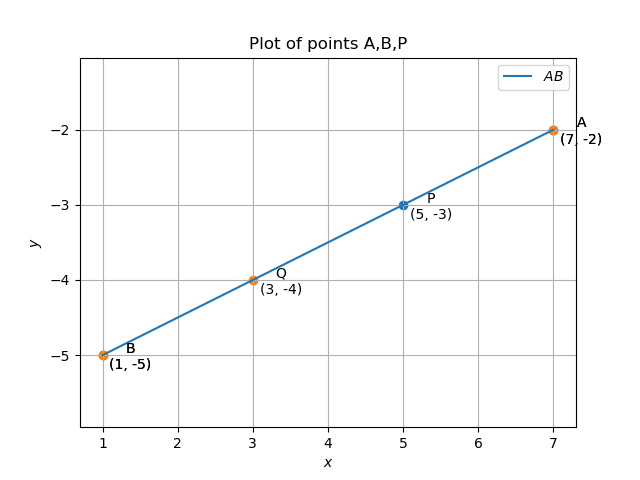
\includegraphics[width=0.7\textwidth]{figs/figasgn2.png}
\end{figure}
\end{document}

